

\title{Schlüsselexperimente in der Teilchenphysik}
\author{
        Jean-Marco Alameddine \\
}
\date{\today}

\documentclass[12pt]{article}

% deutsche Spracheinstellungen
\usepackage{polyglossia}
\setmainlanguage{german}

\usepackage{suffix}

\usepackage{geometry}
\geometry{a4paper,left=25mm,right=25mm, top=3cm, bottom=3cm}

% unverzichtbare Mathe-Befehle
\usepackage{amsmath}
% viele Mathe-Symbole
\usepackage{amssymb}
% Erweiterungen für amsmath
\usepackage{mathtools}

% Fonteinstellungen
\usepackage{fontspec}
% Latin Modern Fonts werden automatisch geladen

\usepackage[
  math-style=ISO,    % ┐
  bold-style=ISO,    % │
  sans-style=italic, % │ ISO-Standard folgen
  nabla=upright,     % │
  partial=upright,   % ┘
  warnings-off={           % ┐
    mathtools-colon,       % │ unnötige Warnungen ausschalten
    mathtools-overbracket, % │
  },                       % ┘
]{unicode-math}

% traditionelle Fonts für Mathematik
\setmathfont{Latin Modern Math}
\setmathfont{XITS Math}[range={scr, bfscr}]
\setmathfont{XITS Math}[range={cal, bfcal}, StylisticSet=1]

% Zahlen und Einheiten
\usepackage[
  locale=DE,                 % deutsche Einstellungen
  separate-uncertainty=true, % immer Fehler mit \pm
  per-mode=reciprocal,       % ^-1 für inverse Einheiten
  % alternativ:
  % per-mode=reciprocal, % m s^{-1}
  % decimal-marker=., % . statt , f�r Dezimalzahlen
]{siunitx}


% Grafiken können eingebunden werden
\usepackage{graphicx}
% größere Variation von Dateinamen möglich (Probleme mit Leerzeichen behoben)
\usepackage{grffile}

\usepackage{float}

\newcommand\chapterauthor[1]{\authortoc{#1}\printchapterauthor{#1}}
\WithSuffix\newcommand\chapterauthor*[1]{\printchapterauthor{#1}}

\makeatletter
\newcommand{\printchapterauthor}[1]{%
  {\parindent0pt\vspace*{-25pt}%
  \linespread{1.5}\large\scshape#1%
  \par\nobreak\vspace*{35pt}}
  \@afterheading%
}
\newcommand{\authortoc}[1]{%
  \addtocontents{toc}{\vskip-5pt}%
  \addtocontents{toc}{%
    \protect\contentsline{chapter}%
    {\hskip1.3em\mdseries\scshape\protect\scriptsize#1}{}{}}
  \addtocontents{toc}{\vskip5pt}%
}
\makeatother

\begin{document}

\maketitle
\newpage

%\begin{abstract}
%This is the paper's abstract \ldots
%\end{abstract}

\tableofcontents
\newpage

\section{Cherenkov-Detektoren}

\chapterauthor{Rune Dominik, 26.10.2018}

\subsection{Geschichte}
Tatsächlich hat bereits Marie Curie blaues Licht gesehen, was heute als Cherenkovlicht erklärt werden kann.

\subsection{Theorie}
Der Cherenkoveffekt tritt auf, wenn geladene Teilchen mit Überlichtgeschwindigkeit durch ein Medium propagieren. Es wird hierdurch ein Cherekovlichtkegel abgegeben, siehe Abbildung \ref{fig:aufbau}.

\begin{figure}[H]
  \centering
  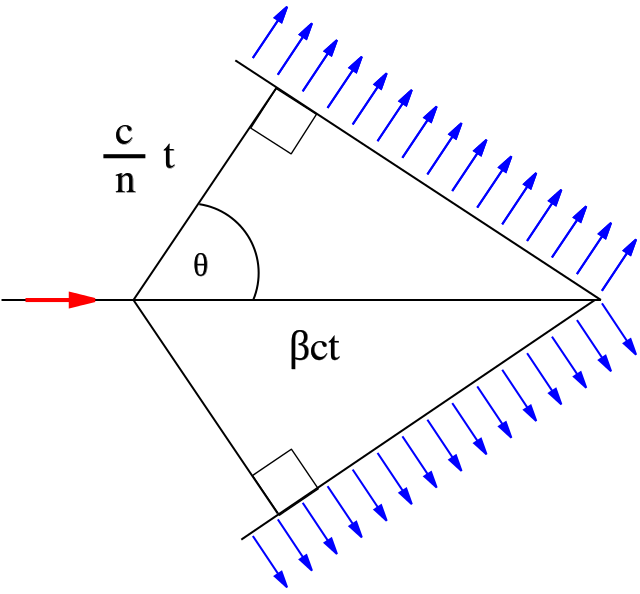
\includegraphics[height=6.0cm]{content/Cherenkov.png}
  \caption{Theoretische Erklärung des Cherenkoveffektes.}
  \label{fig:aufbau}
\end{figure}

\subsection{Aufbau}
Es gibt verschiedene Bauweisen für solche Teleskope. Insbesondere die HESE ist eine sehr moderne Bauweise.

Test~\cite{Gil:02}



\newpage

\bibliographystyle{abbrv}
\bibliography{summary}

\end{document}

